\documentclass[border=5pt]{standalone}
\usepackage{tikz}
\usepackage{amsmath}
\usetikzlibrary{matrix,positioning}

\begin{document}
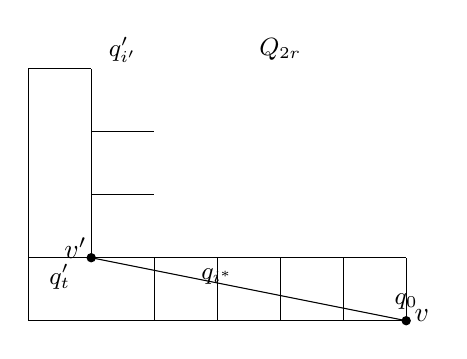
\begin{tikzpicture}[scale=0.8]
  % 定义样式
  \tikzset{
    grid point/.style={circle, fill, inner sep=1.2pt},
    math label/.style={font=\small}
  }
  
  % 创建垂直网格部分
  \draw (0,0) -- (0,4);
  \draw (0,4) -- (1,4);
  \draw (1,1) -- (1,4);
  \draw (0,1) -- (0,0) -- (6,0);
  
  % 创建水平网格部分
  \draw (0,1) -- (6,1);
  \foreach \i in {2,...,6} {
    \draw (\i,0) -- (\i,1);
  }
  
  % 创建垂直小方格
  \foreach \i in {2,3} {
    \draw (1,\i) -- (2,\i);
  }
  \draw (1,1) -- (2,1);
  
  % 添加对角线
  \draw (1,1) -- (6,0);
  
  % 添加标记点
  \node[grid point, label={[xshift=-0.2cm, yshift=-0.2cm]:$v'$}] at (1,1) {};
  \node[grid point, label={[xshift=0.2cm, yshift=-0.2cm]:$v$}] at (6,0) {};
  
  % 添加标签
  \node[math label] at (1.5,4.3) {$q'_{i'}$};
  \node[math label] at (4,4.3) {$Q_{2r}$};
  \node[math label] at (0.5,0.7) {$q'_t$};
  \node[math label] at (3,0.7) {$q_{i^*}$};
  \node[math label] at (6,0.3) {$q_0$};
\end{tikzpicture}
\end{document}